\documentclass[tikz,border=8pt]{standalone}
\usetikzlibrary{arrows.meta,positioning}
\begin{document}
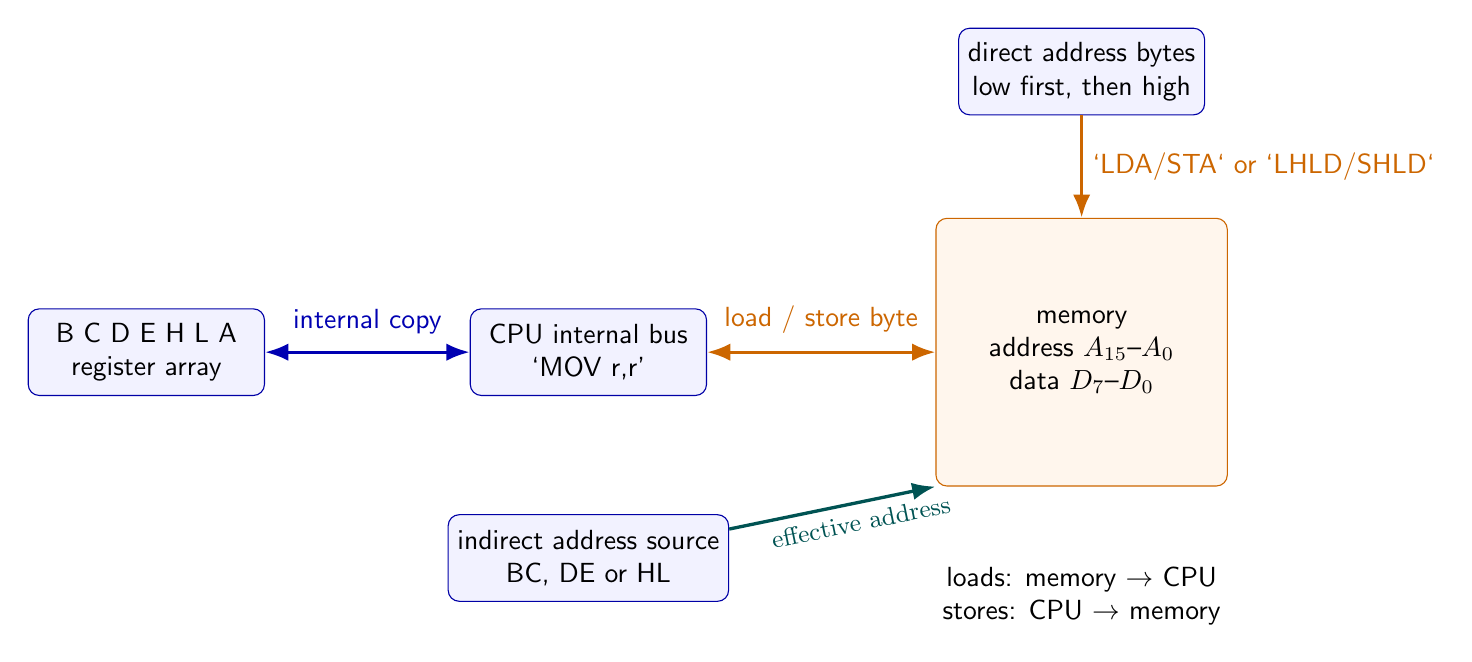
\begin{tikzpicture}[font=\sffamily,>=Latex,node distance=8mm and 14mm,
box/.style={draw=blue!65!black,rounded corners,fill=blue!5,minimum width=30mm,minimum height=11mm,align=center},
mem/.style={draw=orange!80!black,rounded corners,fill=orange!7,minimum width=37mm,minimum height=34mm,align=center},
arr/.style={<->,very thick}]
\node[box] (regs) {B C D E H L A\\register array};
\node[box,right=26mm of regs] (ibus) {CPU internal bus\\`MOV r,r'};
\node[mem,right=29mm of ibus] (memory) {memory\\address $A_{15}$--$A_0$\\data $D_7$--$D_0$};
\node[box,below=15mm of ibus] (pairs) {indirect address source\\BC, DE or HL};
\node[box,above=13mm of memory] (inst) {direct address bytes\\low first, then high};
\draw[arr,blue!70!black] (regs)--node[above=5pt,fill=white,inner sep=1pt]{internal copy}(ibus);
\draw[arr,orange!80!black] (ibus)--node[above=5pt,fill=white,inner sep=1pt]{load / store byte}(memory);
\draw[->,very thick,teal!65!black] (pairs)--node[pos=.62,below,sloped,font=\small]{effective address}(memory.south west);
\draw[->,very thick,orange!80!black] (inst)--node[right]{`LDA/STA` or `LHLD/SHLD`}(memory);
\node[below=9mm of memory,align=center] {loads: memory $\rightarrow$ CPU\\stores: CPU $\rightarrow$ memory};
\end{tikzpicture}
\end{document}
